% Sections/07_xai.tex
% Explainable AI (XAI) Analysis Section

\section{Explainable AI (XAI) Analysis}
\label{sec:xai}

To understand how the centralized and federated architectures utilize physical features, we apply SHAP (SHapley Additive exPlanations) and LIME (Local Interpretable Model-agnostic Explanations) on our models.

\subsection{Global Interpretability (SHAP)}
\label{subsec:global_interpret}

SHAP analysis identifies key features driving model classifications across the global dataset. The SHAP summary plots in Figure 9 compare the feature importance of the Federated + DP model against the Centralized + DP model~\cite{lundberg2017unified}:

\begin{figure}[htbp]
  \centering
  \begin{subfigure}[b]{0.48\textwidth}
    \centering
    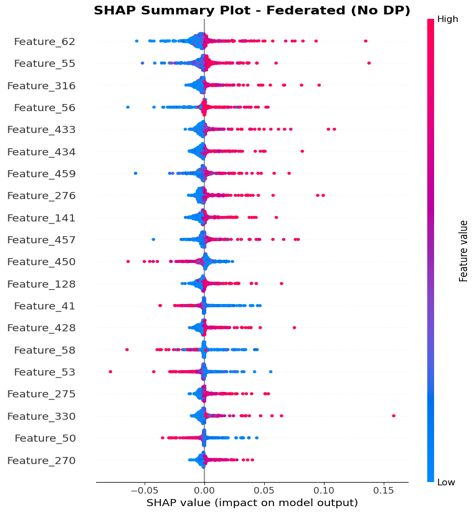
\includegraphics[width=\textwidth]{figures/fig9a.png}
    \caption{Federated + DP model}
    \label{fig:shap_fl_dp}
  \end{subfigure}
  \hfill
  \begin{subfigure}[b]{0.48\textwidth}
    \centering
    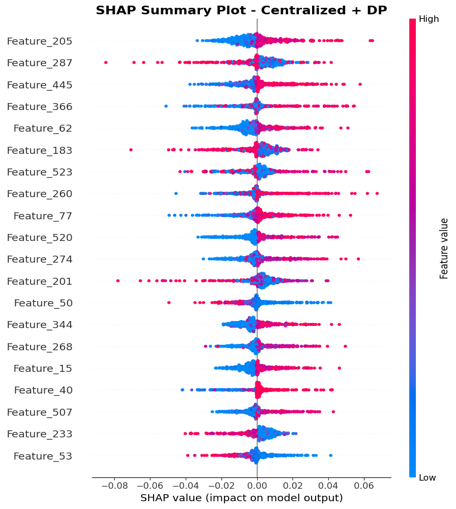
\includegraphics[width=\textwidth]{figures/fig9b.png}
    \caption{Centralized + DP model}
    \label{fig:shap_cl_dp}
  \end{subfigure}
  \caption{SHAP feature importance comparison between FL + DP (left) and Centralized + DP (right)}
  \label{fig:shap_comparison}
\end{figure}

The SHAP summary plots show that both models prioritize high-frequency signals and variance in accelerometer data for dynamic activities, and gravity-based signals for static behaviors (laying/sitting). However, the FL+DP model exhibits slightly more distributed importance across a wider subset of features, a regularization effect of federated client partitioning and DP noise. This suggests that federated training prevents individual clients' dominant features from over-influencing the global model, promoting broader generalization.

\subsection{Local Interpretability (LIME)}
\label{subsec:local_interpret}

LIME provides instance-level explanations of single activity predictions, showing the contribution of individual features towards classification decisions~\cite{ribeiro2016why}:

\begin{figure}[htbp]
  \centering
  \begin{subfigure}[b]{0.48\textwidth}
    \centering
    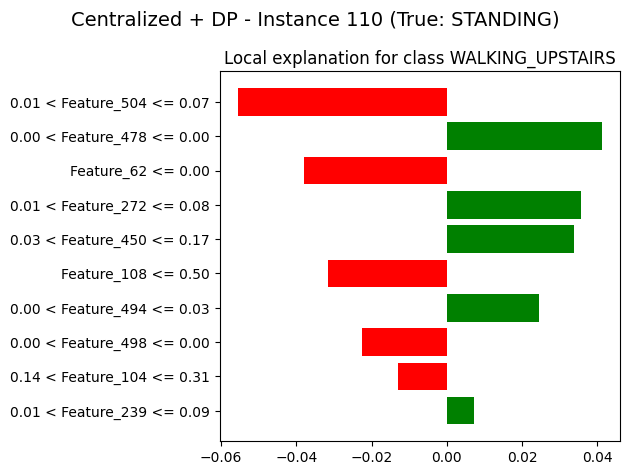
\includegraphics[width=\textwidth]{figures/fig10a.png}
    \caption{Centralized standing prediction}
    \label{fig:lime_central}
  \end{subfigure}
  \hfill
  \begin{subfigure}[b]{0.48\textwidth}
    \centering
    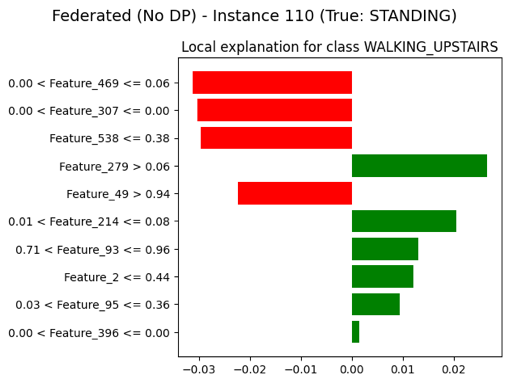
\includegraphics[width=\textwidth]{figures/fig10b.png}
    \caption{Federated standing prediction}
    \label{fig:lime_federated}
  \end{subfigure}
  \caption{LIME instance explanations for Centralized (left) and Federated (right) standing prediction}
  \label{fig:lime_comparison}
\end{figure}

For standing predictions, the centralized model relies on a few key gravity features (gravityMean-X, gravityMean-Y) to make highly confident predictions. In contrast, the federated model's decision boundary is shaped by a more diverse collection of features with lower individual weights, demonstrating a more stable, ensemble-like prediction behavior. This aligns with the federated architecture's design of aggregating model weights from diverse clients, which implicitly averages out local subject biases.
